\chapter{排序算法}

\section{希尔排序}

\subsection{希尔排序(Shell Sort)}

希尔排序本质上是直接插入排序的升级版。对于插入排序而言,在大多数元素已经有序的情况下,工作量会比较小。这个结论很明显,如果一个数组大部分元素都有序,那么数组中的元素自然不需要频繁地进行比较和交换。\\

如何能够让待排序的数组中大部分元素有序呢?需要对原始数组进行预处理,使得原始数组的大部分元素变得有序。采用分组的方法,可以将数组进行一定程度地粗略调整。\\

例如一个有8个数字组成的无序序列\{5, 8, 6, 3, 9, 2, 1, 7\},进行升序排序。让元素两两一组,同组两个元素之间的跨度为数组总长度的一半。\\

接着让每组元素进行独立排序,排序方式使用直接插入排序即可。由于每一组的元素数量很少,所以插入排序的工作量很少。这样一来,仅仅经过几次简单的交换,数组整体的有序程序得到了显著提高,使得后续再进行直接插入排序的工作量大大减少。\\

但是这样还不算完,还可以进一步缩小分组跨度,重复上述工作。\\

例如一个有8个数字组成的无序序列\{5, 8, 6, 3, 9, 2, 1, 7\},进行升序排序。

\begin{figure}[H]
	\centering
	\begin{tikzpicture}[font=\ttfamily,
			array/.style={matrix of nodes,nodes={draw, minimum size=10mm, fill=green!30},column sep=-\pgflinewidth, row sep=0.5mm, nodes in empty cells,
					row 1/.style={nodes={draw=none, fill=none, minimum size=5mm}},
				}]

		\matrix[array] (array) {
			0 & 1 & 2 & 3 & 4 & 5 & 6 & 7 \\
			5 & 2 & 1 & 3 & 9 & 8 & 6 & 7 \\
		};

		\draw[-, red] (-3.5,-0.8) -- (-3.5,-1.2) -- (0.5,-1.2) -- (0.5,-0.8);
		\draw[-, red] (-2.5,-0.8) -- (-2.5,-1.4) -- (1.5,-1.4) -- (1.5,-0.8);
		\draw[-, red] (-1.5,-0.8) -- (-1.5,-1.6) -- (2.5,-1.6) -- (2.5,-0.8);
		\draw[-, red] (-0.5,-0.8) -- (-0.5,-1.8) -- (3.5,-1.8) -- (3.5,-0.8);
	\end{tikzpicture}
	\caption{跨度为4分组交换}
\end{figure}

\begin{figure}[H]
	\centering
	\begin{tikzpicture}[font=\ttfamily,
			array/.style={matrix of nodes,nodes={draw, minimum size=10mm, fill=green!30},column sep=-\pgflinewidth, row sep=0.5mm, nodes in empty cells,
					row 1/.style={nodes={draw=none, fill=none, minimum size=5mm}},
				}]

		\matrix[array] (array) {
			0 & 1 & 2 & 3 & 4 & 5 & 6 & 7 \\
			1 & 2 & 5 & 3 & 6 & 7 & 9 & 8 \\
		};

		\draw[-, red] (-3.5,-0.8) -- (-3.5,-1.2) -- (-1.6,-1.2) -- (-1.6,-0.8);
		\draw[-, red] (-2.5,-0.8) -- (-2.5,-1.4) -- (-0.6,-1.4) -- (-0.6,-0.8);
		\draw[-, red] (-1.5,-0.8) -- (-1.5,-1.6) -- (0.4,-1.6) -- (0.4,-0.8);
		\draw[-, red] (-0.5,-0.8) -- (-0.5,-1.2) -- (1.4,-1.2) -- (1.4,-0.8);
		\draw[-, red] (0.5,-0.8) -- (0.5,-1.4) -- (2.5,-1.4) -- (2.5,-0.8);
		\draw[-, red] (1.5,-0.8) -- (1.5,-1.6) -- (3.5,-1.6) -- (3.5,-0.8);
	\end{tikzpicture}
	\caption{跨度为2分组交换}
\end{figure}

\begin{figure}[H]
	\centering
	\begin{tikzpicture}[font=\ttfamily,
			array/.style={matrix of nodes,nodes={draw, minimum size=10mm, fill=green!30},column sep=-\pgflinewidth, row sep=0.5mm, nodes in empty cells,
					row 1/.style={nodes={draw=none, fill=none, minimum size=5mm}},
				}]

		\matrix[array] (array) {
			0 & 1 & 2 & 3 & 4 & 5 & 6 & 7 \\
			1 & 2 & 3 & 5 & 6 & 7 & 8 & 9 \\
		};
	\end{tikzpicture}
	\caption{跨度为1分组交换}
\end{figure}

希尔排序的发明者是计算机科学家Donald Shell。希尔排序中说使用的分组跨度被称为希尔排序的增量。增量的选择可以有很多种,最朴素的就是Donald Shell在发明希尔排序时所提出的逐步折半的方法。\\

\mybox{希尔排序}

\begin{lstlisting}[language=C]
void shellSort(int *arr, int n) {
    int gap = n;
    while(gap > 1) {
        gap /= 2;
        for(int i = 0; i < gap; i++) {
            for(int j = i+gap; j < n; j += gap) {
                int temp = arr[j];
                int k = j - gap;
                while(k >= 0 && arr[k] > temp) {
                    arr[k+gap] = arr[k];
                    k -= gap;
                }
                arr[k+gap] = temp;
            }
        }
    }    
}
\end{lstlisting}

\vspace{0.5cm}

\subsection{算法分析}

希尔排序利用分组粗略调整的方式减少了直接插入排序的工作量,使得算法的平均时间复杂度低于$ O(n^2) $。但是在某些极端情况下,希尔排序的最坏时间复杂度仍然是$ O(n^2) $,甚至比插入排序更慢。\\

例如\{2, 1, 5, 3, 7, 6, 9, 8\},无论是以4为增量,还是以2为增量,每组内部的元素都没有任何交换。直到增量缩减为1,数组才会按照直接插入排序的方式进行调整。\\

对于这样的数组,希尔排序不但没有减少直接插入排序的工作量,反而白白增加了分组操作的成本。\\

这是因为每一轮希尔增量之间都是等比的,这就导致了希尔增量存在盲区。为了避免这样的极端情况,科学家发明了许多更为严谨的增量方式。其中最具有代表性的是Hibbard增量和Sedgewick增量。

\subsubsection{Hibbard增量序列}

Hibbard增量序列为$ 1, 3, 7, 15, \dots $,通项公式为$ 2^i - 1 $。\\

利用这种增量方式的希尔排序,最坏时间复杂度是$ O(n^{3/2}) $。\\

\mybox{Hibbard增量序列}

\begin{lstlisting}[language=Python]
def get_hibbard_sequence(n):
    """
        生成Hibbard序列
        1, 3, 7, 15, 31, 63, ...
    """
    sequence = []
    i = 1
    while i <= n:
        sequence.append(i)
        i = (i << 1) + 1
    sequence.reverse()
    return sequence

def shell_sort_hibbard(lst):
    """
        希尔排序(Hibbard增量序列)
    """
    n = len(lst)
    hibbard = get_hibbard_sequence(n)
    for gap in hibbard:
        for i in range(gap, n):
            j = i
            temp = lst[j]
            while j >= gap:
                if temp < lst[j-gap]:
                    lst[j] = lst[j-gap]
                    j -= gap
                else:
                    break
            lst[j] = temp
\end{lstlisting}

\subsubsection{Sedgewick增量序列}

Sedgewick增量序列为$ 1, 5, 19, 41, 109, \dots $,通项公式为$ 9 \times 4^i - 9 \times 2^i + 1 $和$ 4^{i+2} - 3 \times 2^{i+2} + 1 $。\\

利用这种增量方式的希尔排序,最坏时间复杂度是$ O(n^{4/3}) $。\\

\mybox{Sedgewick增量序列}

\begin{lstlisting}[language=Python]
def get_sedgewick_sequence(n):
    """
        生成Sedgewick序列
        1, 5, 19, 41, 109, ...
    """
    sequence = []
    i = 0
    while True:
        # 9 * 4^i - 9 * 2^i + 1
        # ==> 9 * (2^(2*i) - 2^i) + 1
        item = 9 * ((1 << (2 * i)) - (1 << i)) + 1
        if item <= n:
            sequence.append(item)
        else:
            break

        # 4^(i+2) - 3 * 2^(i+2) + 1
        # ==> 2^(2i+4) - 3 * 2^(i+2) + 1
        item = (1 << (2 * i + 4)) - 3 * (1 << (i + 2)) + 1
        if item <= n:
            sequence.append(item)
        else:
            break
        
        i += 1
    return sequence

def shell_sort_sedgewick(lst):
    """
        希尔排序(Sedgewick增量序列)
    """
    n = len(lst)
    sedgewick = get_sedgewick_sequence(n)
    for gap in sedgewick:
        for i in range(gap, n):
            j = i
            temp = lst[j]
            while j >= gap:
                if temp < lst[j-gap]:
                    lst[j] = lst[j-gap]
                    j -= gap
                else:
                    break
            lst[j] = temp
\end{lstlisting}

这两种增量方式的时间复杂度需要很复杂的数学证明,有些是人们的大致猜想。

\begin{table}[H]
	\centering
	\setlength{\tabcolsep}{5mm}{
		\begin{tabular}{|c|c|c|}
			\hline
			\textbf{时间复杂度}   & \textbf{空间复杂度} & \textbf{稳定性} \\
			\hline
			$ O(n^{1.3 \sim 2}) $ & $ O(1) $            & 不稳定          \\
			\hline
		\end{tabular}
	}
	\caption{希尔排序算法分析}
\end{table}

\newpage

\section{归并排序}

\subsection{归并排序优化}

简单的归并排序利用分治法,递归地将对小规模子数组进行处理。但是递归会使小规模问题中方法调用太过频繁,因此对于规模较小的子数组可以采用插入排序。一般来说插入排序在小数组中比归并更快,这种优化可以使归并排序的运行时间缩短10\% $ \sim $ 15\%。\\

另一个可以优化的地方是对于单次合并的过程,例如将子数组$ arr[start..mid] $和$ arr[mid+1..end] $进行合并,如果$ arr[mid] \le arr[mid+1] $的话,说明$ arr[start..end] $已经为有序状态,无序再进行不必要的合并。\\

\mybox{归并排序优化}

\begin{lstlisting}[language=C]
void mergeSortWorker(int *arr, int start, int end, int *temp) {
    // 列表长度小于10时,采用二分插入排序
    if(end - start <= 10) {
        binaryInsertionSort(arr, start, end);
        return;
    }
    if(start < end) {
        int mid = start + (end - start) / 2;
        mergeSortWorker(arr, start, mid, temp);
        mergeSortWorker(arr, mid+1, end, temp);
        // 避免不必要的合并
        if(arr[mid] <= arr[mid+1]) {
            return;
        }
        merge(arr, start, mid, end, temp);
    }
}
\end{lstlisting}

\vspace{0.5cm}

\subsection{归并排序迭代实现}

递归实现的归并排序是自顶向下的过程,基于循环的归并排序是自底向上进行的。非递归的归并排序避免了递归时深度为$ logn $的栈空间,空间上只用到了长度为n的临时空间。\\

\mybox{归并排序(迭代)}

\begin{lstlisting}[language=Java]
public static void mergeSort(int[] arr) {
    int n = arr.length;
    int[] temp = new int[n];
    int pos = 0;            // 临时数组的下表
    int left1, left2;       // 左子数组边界
    int right1, right2;     // 右子数组边界

    for (int i = 1; i < n; i *= 2) {
        for (left1 = 0; left1 < n - i; left1 = right2) {
            // 设置子数组边界
            right1 = left2 = left1 + i;
            right2 = left2 + i;

            // 防止右边界越界
            right2 = right2 > n ? n : right2;

            pos = 0;
            while (left1 < left2 && right1 < right2) {
                if (arr[left1] < arr[right1]) {
                    temp[pos++] = arr[left1++];
                } else {
                    temp[pos++] = arr[right1++];
                }
            }

            while (left1 < left2) {
                arr[--right1] = arr[--left2];
            }

            // 将排好序的部分保存回数组
            while (pos > 0) {
                arr[--right1] = temp[--pos];
            }
        }
    }
}
\end{lstlisting}

\vspace{0.5cm}

\subsection{外部排序}

在内存中进行的排序称为内部排序,而在许多实际应用中,经常需要对大文件进行排序。因为文件中的信息量庞大,无法将整个文件拷贝进内存进行排序。因此需要将待排序的记录存储在外存上,排序时再把数据一部分一部分调入内存进行排序,再讲排好序的记录写回文件中。\\

因为磁盘读写的时间远超过内存计算的时间,因此外部排序过程中的时间代价主要是磁盘I/O次数。\\

假如需要对一个包含40亿个int类型整数的文件进行排序,而计算机的内存只有2GB。一个int占4个字节,40亿个需要160亿字节,大概占用8GB的内存。因此可以把8GB分割成4份2GB的数据进行排序,然后再把它们凑回去。\\

\begin{figure}[H]
	\centering
	\begin{tikzpicture}
		\draw (0,0) rectangle node{8G无序数据} (3,2);
		\draw (1.5,2.5) node{硬盘文件};
		\draw (5,0) rectangle node{2G内存} (7,2);
		\draw (9,-1) rectangle (12,3);
		\draw (9,0) -- (12,0);
		\draw (9,1) -- (12,1);
		\draw (9,2) -- (12,2);
		\draw (10.5,-0.5) node{2G有数数据};
		\draw (10.5,0.5) node{2G有数数据};
		\draw (10.5,1.5) node{2G有数数据};
		\draw (10.5,2.5) node{2G有数数据};

		\draw[->] (3,1) -- (4,1) node[above]{加载} -- (5,1);
		\draw[->] (7,1) -- (8,1) node[above]{排序} -- (9,1);
	\end{tikzpicture}
	\caption{分割数据}
\end{figure}

排序的时候可以采用归并排序,每次将两个有序子串合并层一个大的有序子串。\\

\begin{figure}[H]
	\centering
	\begin{tikzpicture}
		\draw (0,0) rectangle (3,2);
		\draw (0,1) -- (3,1);
		\draw (1.5,1.5) node{2G有序数据};
		\draw (1.5,0.5) node{2G有序数据};
		\draw (5,0) rectangle node{2G内存} (7,2);
		\draw (9,0.5) rectangle (12,1.5);
		\draw (10.5,1) node{4G有序数据};

		\draw[->] (3,1) -- (4,1) node[above]{读取} -- (5,1);
		\draw[->] (7,1) -- (8,1) node[above]{写入硬盘} -- (9,1);
	\end{tikzpicture}
	\caption{二路归并}
\end{figure}

不过硬盘的读写速度比内存要慢得多,通过优化可以降低数据从硬盘读写的次数。\\

在进行有序数据合并的时候,不采取两两合并的方法,而是可以三组或四组数据一起合并。n个有序数据的合并被称为n路归并。

\newpage

\section{快速排序}

\subsection{随机选择基准值}

快速排序利用分治法,通过一趟排序将数组分为两部分,其中一部分小于等于基准值,另一部分大于等于基准值,然后再递归对两个子问题排序。\\

基本的快速排序采用序列的第一个元素作为基准值,但是这不是一种好方法。当数组已经有序时,这样的分割效率非常糟糕。为了缓解这种极端情况,可以在待排序数组中随机选择一个元素作为基准值。\\

\mybox{随机选取基准值}

\begin{lstlisting}[language=C]
int selectRandomPivot(int *arr, int start, int end) {
    srand(time(NULL));
    int pos = rand() % (end - start) + start;
    swap(&arr[pos], &arr[start]);
    return arr[start];
}
\end{lstlisting}

\vspace{0.5cm}

\subsection{三数取中}

虽然随机选取基准值可以减少出现分割不好的几率,但是最坏情况下还是$ O(n) $。另一种选取基准值的方法就是三数取中,也就是取序列中start、mid、end三个元素的中间值作为基准值。\\

\mybox{三数取中}

\begin{lstlisting}[language=C]
int selectMedianPivot(int *arr, int start, int end) {
    int mid = start + (end - start) / 2;
    if(arr[mid] > arr[end]) {
        swap(&arr[mid], &arr[end]);
    }
    if(arr[start] > arr[end]) {
        swap(&arr[start], &arr[end]);
    }
    if(arr[mid] > arr[start]) {
        swap(&arr[mid], &arr[start]);
    }
    // 此时arr[mid] <= arr[start] <= arr[end]
    return arr[start];
}
\end{lstlisting}

\vspace{0.5cm}

\subsection{三数取中+插入排序}

对于很小和部分有序的数组,快速排序的效率不如插入排序。因此当待排序数组被分割到一定大小后,可直接采用插入排序。\\

\mybox{三数取中+插入排序}

\begin{lstlisting}[language=C]
void quickSort(int *arr, int start, int end) {
    if(end - start <= 10) {
        binaryInsertionSort(arr, start, end);
        return;
    }
    
    if(start < end) {
        int i = start;
        int j = end;
        int pivot = selectMedianPivot(arr, start, end);

        while(i < j) {
            while(i < j && arr[j] > pivot) {
                j--;
            }
            if(i < j) {
                arr[i] = arr[j];
                i++;
            }
            while(i < j && arr[i] < pivot) {
                i++;
            }
            if(i < j) {
                arr[j] = arr[i];
                j--;
            }
        }
        arr[i] = pivot;
        quickSort(arr, start, i-1);
        quickSort(arr, i+1, end);
    } 
}
\end{lstlisting}

\vspace{0.5cm}

\subsection{聚集相等基准值}

在一次分割结束后,可以把所有与基准值相等的元素聚集在一起,这样在下次分割时,就不用对这些值再分割了。\\

例如待排序序列为\{1, 4, 6, 7, 6, 6, 7, 6, 8, 6\},选择6(下标为4)作为基准值。在进行一次分割后,得到两个子序列\{1, 4, 6\}和\{7, 6, 7, 6, 8, 6\}。将所有与基准值相等的元素聚集后,可得到\{1, 4, 6, 6, 6, 6, 6, 7, 8, 7\}。这样下一次分割的子序列可以减少为\{1, 4\}和\{7, 8, 7\}。\\

\mybox{聚集相等基准值}

\begin{lstlisting}[language=C]
/**
 * @brief  聚集相等基准值
 * @param  arr: 待排序数组
 * @param  start: 数组开始位置
 * @param  end: 数组结束位置
 * @param  pivotPos: 基准值下标
 * @param  left: 相等基准值左边界
 * @param  right: 相等基准值右边界
 */
void gather(int *arr, int start, int end, 
            int pivotPos, int *left, int *right) {
    if(start >= end) {
        return;
    }

    int cnt = pivotPos - 1;
    for(int i = pivotPos - 1; i >= start; i--) {
        if(arr[i] == arr[pivotPos]) {
            swap(&arr[i], &arr[cnt]);
            cnt--;
        }
    }
    *left = cnt;

    cnt = pivotPos + 1;
    for(int i = pivotPos + 1; i <= end; i++) {
        if(arr[i] == arr[pivotPos]) {
            swap(&arr[i], &arr[cnt]);
            cnt++;
        }
    }
    *right = cnt;
}
\end{lstlisting}

\vspace{0.5cm}

\subsection{尾递归优化}

快速排序在函数尾部有2次递归操作,可以对其中的尾递归进行优化。因为在第一次递归后,start就没用了,第二次递归可以用循环代替。\\

\mybox{尾递归优化}

\begin{lstlisting}[language=C]
void quickSort(int *arr, int start, int end) {
    if(end - start <= 10) {
        binaryInsertionSort(arr, start, end);
        return;
    }
    
    while(start < end) {
        int i = start;
        int j = end;
        int pivot = selectMedianPivot(arr, start, end);

        while(i < j) {
            while(i < j && arr[j] > pivot) {
                j--;
            }
            if(i < j) {
                arr[i] = arr[j];
                i++;
            }
            while(i < j && arr[i] < pivot) {
                i++;
            }
            if(i < j) {
                arr[j] = arr[i];
                j--;
            }
        }
        arr[i] = pivot;

        // 聚集与基准值相等元素
        int left, right;
        gather(arr, start, end, i, &left, &right);
        
        quickSort(arr, start, left);
        // quickSort(arr, right, end);  // 消除尾递归
        start = right;
    }
}
\end{lstlisting}

其实这种优化编译器会自己进行优化,因此相比不使用优化的方法,运行时间几乎无异。\\

\subsection{快速排序迭代实现}

递归实现主要是在划分子区间,因此可以通过利用栈的特性来保存区间即可,因为递归本身就是压栈的过程。\\

\mybox{快速排序(迭代)}

\begin{lstlisting}[language=C]
int partition(int *arr, int start, int end) {
    int i = start - 1;
    int pivot = arr[end];

    for(int j = start; j < end; j++) {
        if(arr[j] <= pivot) {
            i++;
            swap(&arr[i], &arr[j]);
        }
    }

    swap(&arr[i+1], &arr[end]);
    return i + 1;
}

void quickSort(int *arr, int start, int end) {
    Stack *s = initStack(end - start + 1);
    push(s, start);
    push(s, end);

    while(!isEmptyStack(s)) {
        int right = pop(s);
        int left = pop(s);

        int index = partition(arr, left, right);
        if(index - 1 > left) {
            push(s, left);
            push(s, index - 1);
        }
        if(index + 1 < right) {
            push(s, index + 1);
            push(s, right);
        }
    }
}
\end{lstlisting}

\newpage

\section{堆排序}

\subsection{堆(Heap)}

二叉堆本质上是一种完全二叉树,分为最大堆和最小堆两个类型。在最大堆中,任何一个父结点的值都大于等于它左右孩子结点的值。在最小堆中,任何一个父结点的值都小于等于它左右孩子结点的值。

\begin{figure}[H]
	\centering
	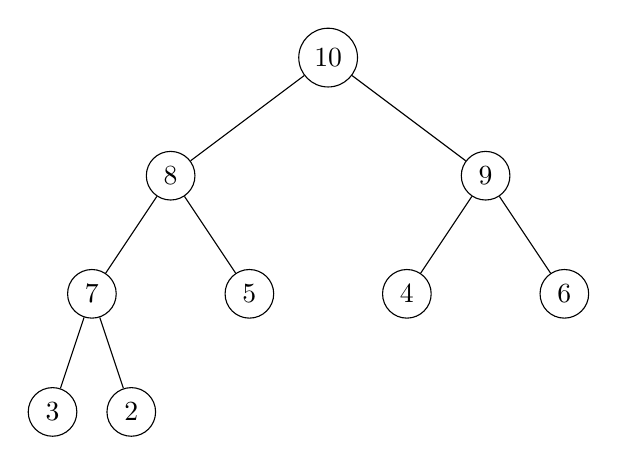
\begin{tikzpicture}[
			level distance=1.5cm,
			level 1/.style={sibling distance=4cm},
			level 2/.style={sibling distance=2cm},
			level 3/.style={sibling distance=1cm}
		]
		\node[circle,draw] {10}
		child {
				node[circle,draw] {8}
				child {
						node[circle,draw] {7}
						child {node[circle,draw] {3}}
						child {node[circle,draw] {2}}
					}
				child {node[circle,draw] {5}}
			}
		child {
				node[circle,draw] {9}
				child {node[circle,draw] {4}}
				child {node[circle,draw] {6}}
			};
	\end{tikzpicture}
	\caption{大顶堆}
\end{figure}

\begin{figure}[H]
	\centering
	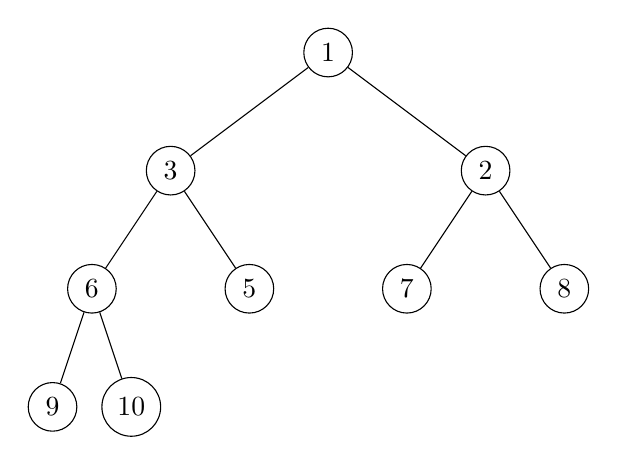
\begin{tikzpicture}[
			level distance=1.5cm,
			level 1/.style={sibling distance=4cm},
			level 2/.style={sibling distance=2cm},
			level 3/.style={sibling distance=1cm}
		]
		\node[circle,draw] {1}
		child {
				node[circle,draw] {3}
				child {
						node[circle,draw] {6}
						child {node[circle,draw] {9}}
						child {node[circle,draw] {10}}
					}
				child {node[circle,draw] {5}}
			}
		child {
				node[circle,draw] {2}
				child {node[circle,draw] {7}}
				child {node[circle,draw] {8}}
			};
	\end{tikzpicture}
	\caption{小顶堆}
\end{figure}

二叉堆的根结点称为堆顶,在最大堆中堆顶是整个堆中的最大元素,在最小堆中堆顶是整个堆中的最小元素。\\

在二叉堆中插入结点、删除结点、构造二叉堆的操作都基于堆的自我调整。\\

二叉堆虽然是一棵完全二叉树,但它的存储方式并不是链式存储,而是顺序存储。数组中,通过下标可以定位到结点的左右孩子,假设父结点的下标是parent,那么它的左孩子下标为2 * parent + 1、右孩子下标为2 * parent + 2。\\

\subsection{插入结点}

二叉堆的插入操作可以看成是结点上浮,当在堆中插入一个结点时,必须满足完全二叉树的标准,那么被插入结点的位置是完全二叉树的最后一个位置。在最大堆中,如果新结点的值大于它的父结点的值,则让新结点上浮,即和父结点交换位置。\\

堆的插入时间复杂度取决于树高为$ O(logn) $。\\

例如在大顶堆\{20, 15, 2, 14, 10\}中插入21:

\begin{figure}[H]
	\centering
	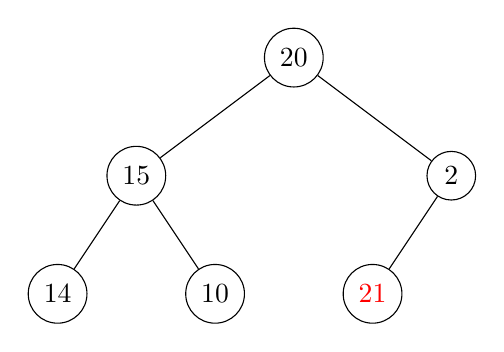
\begin{tikzpicture}[
			level distance=1.5cm,
			level 1/.style={sibling distance=4cm},
			level 2/.style={sibling distance=2cm},
			level 3/.style={sibling distance=1cm}
		]
		\node[circle,draw] {20}
		child {
				node[circle,draw] {15}
				child {node[circle,draw] {14}}
				child {node[circle,draw] {10}}
			}
		child {
				node[circle,draw] {2}
				child {node[circle,draw] {\textcolor{red}{21}}}
				child[missing] {}
			};
	\end{tikzpicture}
\end{figure}

\begin{figure}[H]
	\centering
	\begin{tikzpicture}[font=\ttfamily,
			array/.style={matrix of nodes,nodes={draw, minimum size=10mm, fill=green!30},column sep=-\pgflinewidth, row sep=0.5mm, nodes in empty cells,
					row 1/.style={nodes={draw=none, fill=none, minimum size=5mm}},
				}]

		\matrix[array] (array) {
			0  & 1  & 2 & 3  & 4  & 5                      \\
			20 & 15 & 2 & 14 & 10 & \textcolor{red}{21} \\
		};
	\end{tikzpicture}
\end{figure}

将新元素21与其父结点2比较,因为21 > 2,将21和2的位置交换:

\begin{figure}[H]
	\centering
	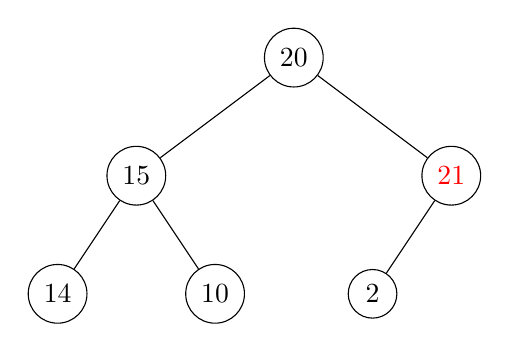
\begin{tikzpicture}[
			level distance=1.5cm,
			level 1/.style={sibling distance=4cm},
			level 2/.style={sibling distance=2cm},
			level 3/.style={sibling distance=1cm}
		]
		\node[circle,draw] {20}
		child {
				node[circle,draw] {15}
				child {node[circle,draw] {14}}
				child {node[circle,draw] {10}}
			}
		child {
				node[circle,draw] {\textcolor{red}{21}}
				child {node[circle,draw] {2}}
				child[missing] {}
			};
	\end{tikzpicture}
\end{figure}

\begin{figure}[H]
	\centering
	\begin{tikzpicture}[font=\ttfamily,
			array/.style={matrix of nodes,nodes={draw, minimum size=10mm, fill=green!30},column sep=-\pgflinewidth, row sep=0.5mm, nodes in empty cells,
					row 1/.style={nodes={draw=none, fill=none, minimum size=5mm}},
				}]

		\matrix[array] (array) {
			0  & 1  & 2                      & 3  & 4  & 5 \\
			20 & 15 & \textcolor{red}{21} & 14 & 10 & 2 \\
		};
	\end{tikzpicture}
\end{figure}

因为21 > 20,将21与20的位置交换:

\begin{figure}[H]
	\centering
	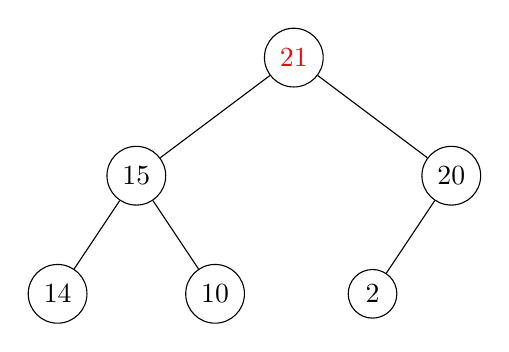
\begin{tikzpicture}[
			level distance=1.5cm,
			level 1/.style={sibling distance=4cm},
			level 2/.style={sibling distance=2cm},
			level 3/.style={sibling distance=1cm}
		]
		\node[circle,draw] {\textcolor{red}{21}}
		child {
				node[circle,draw] {15}
				child {node[circle,draw] {14}}
				child {node[circle,draw] {10}}
			}
		child {
				node[circle,draw] {20}
				child {node[circle,draw] {2}}
				child[missing] {}
			};
	\end{tikzpicture}
\end{figure}

\begin{figure}[H]
	\centering
	\begin{tikzpicture}[font=\ttfamily,
			array/.style={matrix of nodes,nodes={draw, minimum size=10mm, fill=green!30},column sep=-\pgflinewidth, row sep=0.5mm, nodes in empty cells,
					row 1/.style={nodes={draw=none, fill=none, minimum size=5mm}},
				}]

		\matrix[array] (array) {
			0                      & 1  & 2  & 3  & 4  & 5 \\
			\textcolor{red}{21} & 15 & 20 & 14 & 10 & 2 \\
		};
	\end{tikzpicture}
\end{figure}

\vspace{0.5cm}

\subsection{删除结点}

二叉堆的删除操作总是从堆的根结点删除元素。根结点被删除之后为了能够保证该树还是一棵完全二叉树,需要将完全二叉树的最后一个结点补到根结点的位置,让其继续符合完全二叉树的定义。二叉堆的删除结点操作可以看作是结点下沉。在最大堆中,如果新堆顶元素小于它的左右孩子中较大的那个结点,则与它的较大的子结点交换位置。\\

堆的删除时间复杂度取决于树高为$ O(logn) $。\\

例如删除大顶堆的堆顶元素20:

\begin{figure}[H]
	\centering
	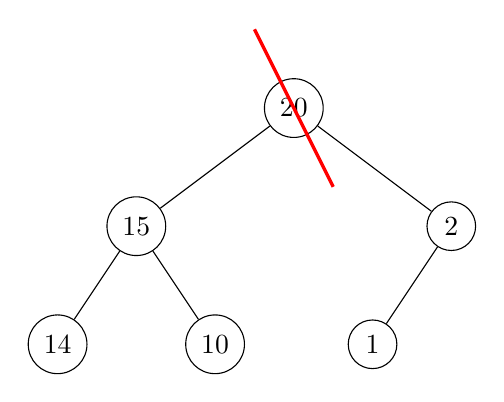
\begin{tikzpicture}[
			level distance=1.5cm,
			level 1/.style={sibling distance=4cm},
			level 2/.style={sibling distance=2cm},
			level 3/.style={sibling distance=1cm}
		]
		\node[circle,draw] {20}
		child {
				node[circle,draw] {15}
				child {node[circle,draw] {14}}
				child {node[circle,draw] {10}}
			}
		child {
				node[circle,draw] {2}
				child {node[circle,draw] {1}}
				child[missing] {}
			};

		\draw[very thick, red] (-0.5,1) -- (0.5,-1);
	\end{tikzpicture}
\end{figure}

\begin{figure}[H]
	\centering
	\begin{tikzpicture}[font=\ttfamily,
			array/.style={matrix of nodes,nodes={draw, minimum size=10mm, fill=green!30},column sep=-\pgflinewidth, row sep=0.5mm, nodes in empty cells,
					row 1/.style={nodes={draw=none, fill=none, minimum size=5mm}},
				}]

		\matrix[array] (array) {
			0                      & 1  & 2 & 3  & 4  & 5 \\
			\textcolor{red}{20} & 15 & 2 & 14 & 10 & 1 \\
		};
	\end{tikzpicture}
\end{figure}

移动最后一个结点到堆顶,使其满足二叉树的性质:

\begin{figure}[H]
	\centering
	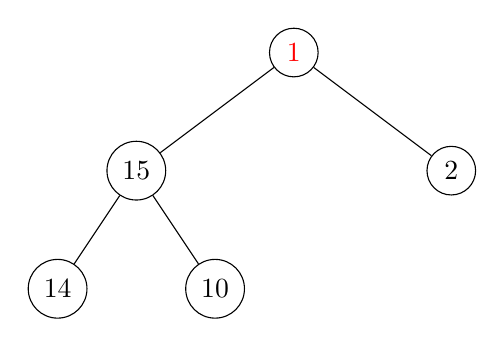
\begin{tikzpicture}[
			level distance=1.5cm,
			level 1/.style={sibling distance=4cm},
			level 2/.style={sibling distance=2cm},
			level 3/.style={sibling distance=1cm}
		]
		\node[circle,draw] {\textcolor{red}{1}}
		child {
				node[circle,draw] {15}
				child {node[circle,draw] {14}}
				child {node[circle,draw] {10}}
			}
		child {node[circle,draw] {2}};
	\end{tikzpicture}
\end{figure}

\begin{figure}[H]
	\centering
	\begin{tikzpicture}[font=\ttfamily,
			array/.style={matrix of nodes,nodes={draw, minimum size=10mm, fill=green!30},column sep=-\pgflinewidth, row sep=0.5mm, nodes in empty cells,
					row 1/.style={nodes={draw=none, fill=none, minimum size=5mm}},
				}]

		\matrix[array] (array) {
			0                      & 1  & 2 & 3  & 4  \\
			\textcolor{red}{1} & 15 & 2 & 14 & 10 \\
		};
	\end{tikzpicture}
\end{figure}

将堆顶元素1与其子结点比较,因为15 > 2,交换较大子结点15与1的位置:

\begin{figure}[H]
	\centering
	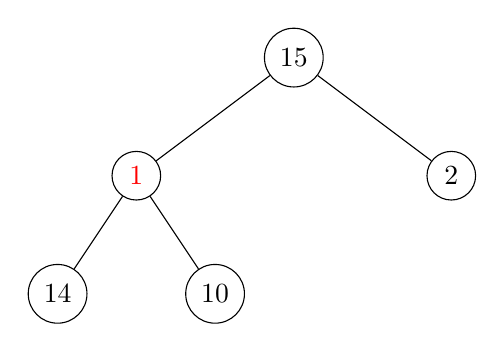
\begin{tikzpicture}[
			level distance=1.5cm,
			level 1/.style={sibling distance=4cm},
			level 2/.style={sibling distance=2cm},
			level 3/.style={sibling distance=1cm}
		]
		\node[circle,draw] {15}
		child {
				node[circle,draw] {\textcolor{red}{1}}
				child {node[circle,draw] {14}}
				child {node[circle,draw] {10}}
			}
		child {node[circle,draw] {2}};
	\end{tikzpicture}
\end{figure}

\begin{figure}[H]
	\centering
	\begin{tikzpicture}[font=\ttfamily,
			array/.style={matrix of nodes,nodes={draw, minimum size=10mm, fill=green!30},column sep=-\pgflinewidth, row sep=0.5mm, nodes in empty cells,
					row 1/.style={nodes={draw=none, fill=none, minimum size=5mm}},
				}]

		\matrix[array] (array) {
			0  & 1                      & 2 & 3  & 4  \\
			15 & \textcolor{red}{1} & 2 & 14 & 10 \\
		};
	\end{tikzpicture}
\end{figure}

继续将元素1与其子结点比较,因为14 > 10,交换较大子结点14与1的位置:

\begin{figure}[H]
	\centering
	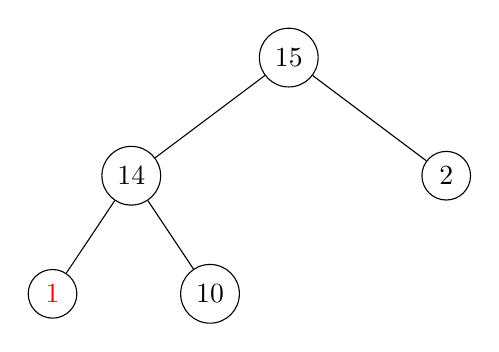
\begin{tikzpicture}[
			level distance=1.5cm,
			level 1/.style={sibling distance=4cm},
			level 2/.style={sibling distance=2cm},
			level 3/.style={sibling distance=1cm}
		]
		\node[circle,draw] {15}
		child {
				node[circle,draw] {14}
				child {node[circle,draw] {\textcolor{red}{1}}}
				child {node[circle,draw] {10}}
			}
		child {node[circle,draw] {2}};
	\end{tikzpicture}
\end{figure}

\begin{figure}[H]
	\centering
	\begin{tikzpicture}[font=\ttfamily,
			array/.style={matrix of nodes,nodes={draw, minimum size=10mm, fill=green!30},column sep=-\pgflinewidth, row sep=0.5mm, nodes in empty cells,
					row 1/.style={nodes={draw=none, fill=none, minimum size=5mm}},
				}]

		\matrix[array] (array) {
			0  & 1 & 2 & 3                      & 4  \\
			15 & 1 & 2 & \textcolor{red}{1} & 10 \\
		};
	\end{tikzpicture}
\end{figure}

\vspace{0.5cm}

\subsection{构建二叉堆}

构建二叉堆,就是把一个无序的完全二叉树调整为二叉堆,本质上就是让所有非叶子结点依次下沉。\\

例如将一个无序的完全二叉树构建成最小堆:

\begin{figure}[H]
	\centering
	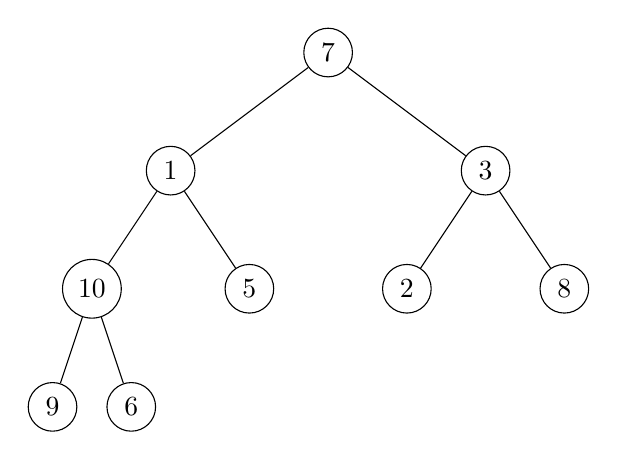
\begin{tikzpicture}[
			level distance=1.5cm,
			level 1/.style={sibling distance=4cm},
			level 2/.style={sibling distance=2cm},
			level 3/.style={sibling distance=1cm}
		]
		\node[circle,draw] {7}
		child {
				node[circle,draw] {1}
				child {
						node[circle,draw] {10}
						child {node[circle,draw] {9}}
						child {node[circle,draw] {6}}
					}
				child {node[circle,draw] {5}}
			}
		child {
				node[circle,draw] {3}
				child {node[circle,draw] {2}}
				child {node[circle,draw] {8}}
			};
	\end{tikzpicture}
\end{figure}

首先从最后一个非叶子结点开始,结点10下沉:

\begin{figure}[H]
	\centering
	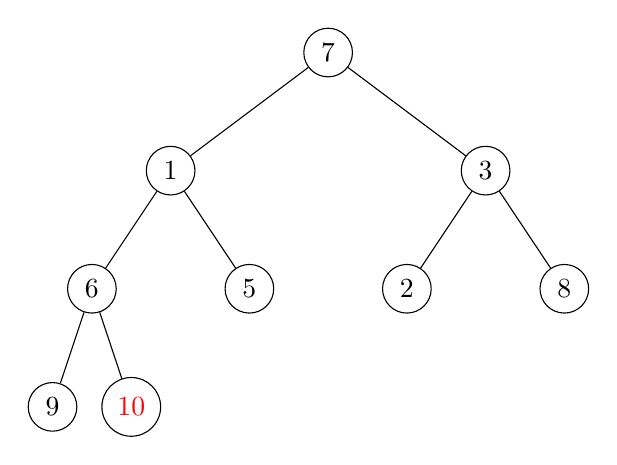
\begin{tikzpicture}[
			level distance=1.5cm,
			level 1/.style={sibling distance=4cm},
			level 2/.style={sibling distance=2cm},
			level 3/.style={sibling distance=1cm}
		]
		\node[circle,draw] {7}
		child {
				node[circle,draw] {1}
				child {
						node[circle,draw] {6}
						child {node[circle,draw] {9}}
						child {node[circle,draw] {\textcolor{red}{10}}}
					}
				child {node[circle,draw] {5}}
			}
		child {
				node[circle,draw] {3}
				child {node[circle,draw] {2}}
				child {node[circle,draw] {8}}
			};
	\end{tikzpicture}
\end{figure}

接着处理倒数第二个非叶子结点,结点3下沉:

\begin{figure}[H]
	\centering
	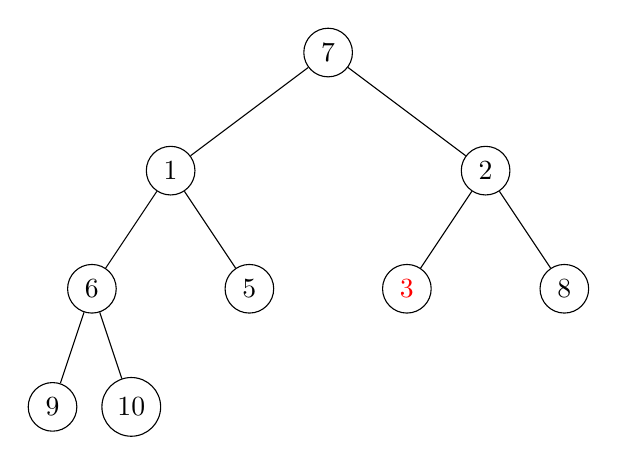
\begin{tikzpicture}[
			level distance=1.5cm,
			level 1/.style={sibling distance=4cm},
			level 2/.style={sibling distance=2cm},
			level 3/.style={sibling distance=1cm}
		]
		\node[circle,draw] {7}
		child {
				node[circle,draw] {1}
				child {
						node[circle,draw] {6}
						child {node[circle,draw] {9}}
						child {node[circle,draw] {10}}
					}
				child {node[circle,draw] {5}}
			}
		child {
				node[circle,draw] {2}
				child {node[circle,draw] {\textcolor{red}{3}}}
				child {node[circle,draw] {8}}
			};
	\end{tikzpicture}
\end{figure}

倒数第三个非叶子结点1无需移动。\\

最后处理倒数第四个非叶子结点7下沉:

\begin{figure}[H]
	\centering
	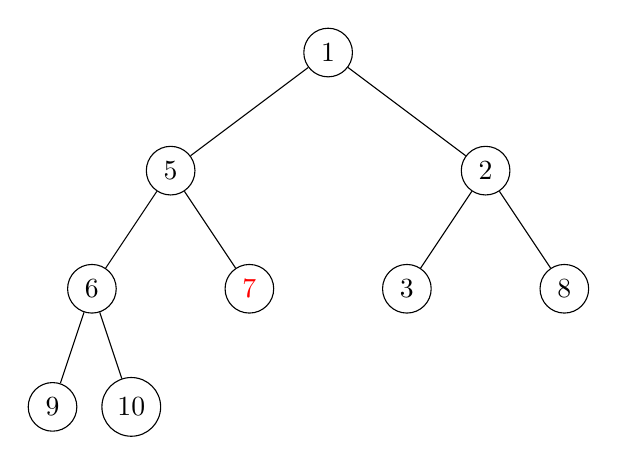
\begin{tikzpicture}[
			level distance=1.5cm,
			level 1/.style={sibling distance=4cm},
			level 2/.style={sibling distance=2cm},
			level 3/.style={sibling distance=1cm}
		]
		\node[circle,draw] {1}
		child {
				node[circle,draw] {5}
				child {
						node[circle,draw] {6}
						child {node[circle,draw] {9}}
						child {node[circle,draw] {10}}
					}
				child {node[circle,draw] {\textcolor{red}{7}}}
			}
		child {
				node[circle,draw] {2}
				child {node[circle,draw] {3}}
				child {node[circle,draw] {8}}
			};
	\end{tikzpicture}
\end{figure}

最终一棵无序完全二叉树就调整成了一个最小堆。\\

\subsection{堆排序(Heap Sort)}

有了二叉堆的构建、删除和自我调节,实现堆排序就是水到聚成了。当删除一个最大堆的堆顶后(并不是完全删除,而是替换到堆的最后面),经过自我调节,第二大的元素就会被交换上来,成为最大堆的新堆顶。\\

首先将待排序数组构建成大顶堆:

\begin{figure}[H]
	\centering
	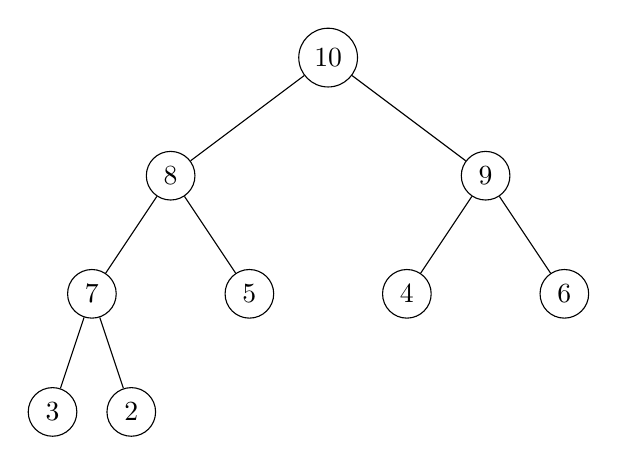
\begin{tikzpicture}[
			level distance=1.5cm,
			level 1/.style={sibling distance=4cm},
			level 2/.style={sibling distance=2cm},
			level 3/.style={sibling distance=1cm}
		]
		\node[circle,draw] {10}
		child {
				node[circle,draw] {8}
				child {
						node[circle,draw] {7}
						child {node[circle,draw] {3}}
						child {node[circle,draw] {2}}
					}
				child {node[circle,draw] {5}}
			}
		child {
				node[circle,draw] {9}
				child {node[circle,draw] {4}}
				child {node[circle,draw] {6}}
			};
	\end{tikzpicture}
\end{figure}

移除堆顶元素(与最后元素交换):

\begin{figure}[H]
	\centering
	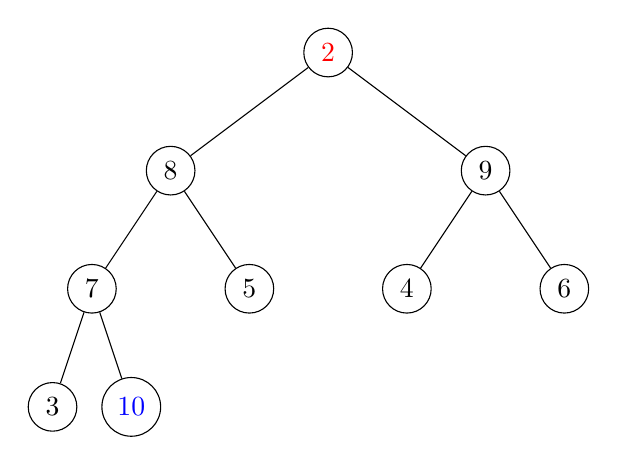
\begin{tikzpicture}[
			level distance=1.5cm,
			level 1/.style={sibling distance=4cm},
			level 2/.style={sibling distance=2cm},
			level 3/.style={sibling distance=1cm}
		]
		\node[circle,draw] {\textcolor{red}{2}}
		child {
				node[circle,draw] {8}
				child {
						node[circle,draw] {7}
						child {node[circle,draw] {3}}
						child {node[circle,draw] {\textcolor{blue}{10}}}
					}
				child {node[circle,draw] {5}}
			}
		child {
				node[circle,draw] {9}
				child {node[circle,draw] {4}}
				child {node[circle,draw] {6}}
			};
	\end{tikzpicture}
\end{figure}

将新的堆顶元素进行下沉,重新调整为大顶堆:

\begin{figure}[H]
	\centering
	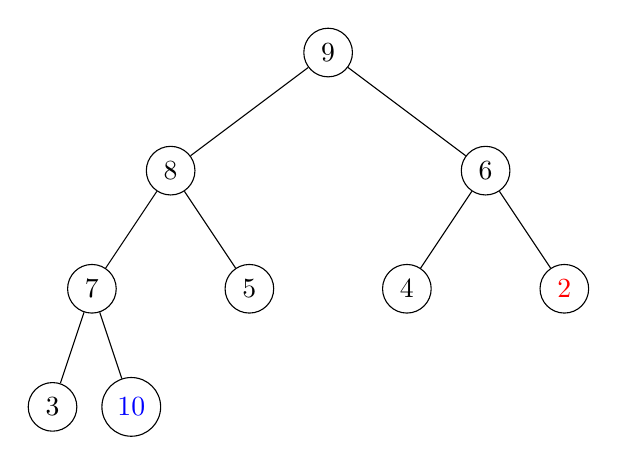
\begin{tikzpicture}[
			level distance=1.5cm,
			level 1/.style={sibling distance=4cm},
			level 2/.style={sibling distance=2cm},
			level 3/.style={sibling distance=1cm}
		]
		\node[circle,draw] {9}
		child {
				node[circle,draw] {8}
				child {
						node[circle,draw] {7}
						child {node[circle,draw] {3}}
						child {node[circle,draw] {\textcolor{blue}{10}}}
					}
				child {node[circle,draw] {5}}
			}
		child {
				node[circle,draw] {6}
				child {node[circle,draw] {4}}
				child {node[circle,draw] {\textcolor{red}{2}}}
			};
	\end{tikzpicture}
\end{figure}

只要反复删除堆顶,反复调节二叉堆,所得到的的集合就成为了一个有序集合。

\begin{figure}[H]
	\centering
	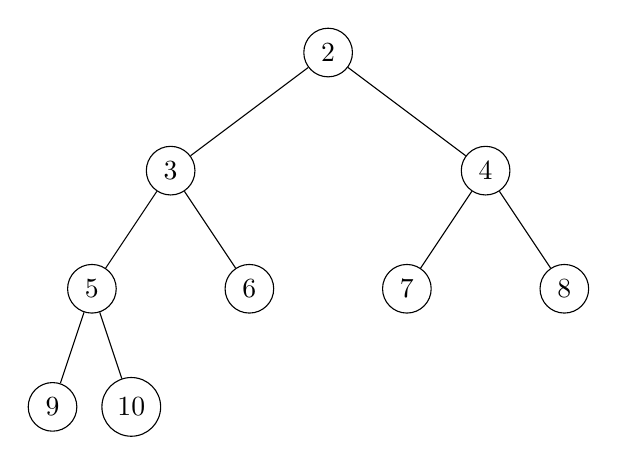
\begin{tikzpicture}[
			level distance=1.5cm,
			level 1/.style={sibling distance=4cm},
			level 2/.style={sibling distance=2cm},
			level 3/.style={sibling distance=1cm}
		]
		\node[circle,draw] {2}
		child {
				node[circle,draw] {3}
				child {
						node[circle,draw] {5}
						child {node[circle,draw] {9}}
						child {node[circle,draw] {10}}
					}
				child {node[circle,draw] {6}}
			}
		child {
				node[circle,draw] {4}
				child {node[circle,draw] {7}}
				child {node[circle,draw] {8}}
			};
	\end{tikzpicture}
\end{figure}

\vspace{0.5cm}

\mybox{堆排序}

\begin{lstlisting}[language=Java]
public static void downAdjust(int[] arr, int parentIndex, int len) {
    // 保存父结点的值,用于最后的赋值
    int temp = arr[parentIndex];
    int childIndex = 2 * parentIndex + 1;

    while(childIndex < len) {
        // 如果有右孩子,且右孩子大于左孩子的值,则定位到右孩子
        if(childIndex + 1 < len 
            && arr[childIndex + 1] > arr[childIndex]) {
            childIndex++;
        }
        // 如果父结点小于任何一个孩子的值,直接跳出
        if(temp >= arr[childIndex]) {
            break;
        }
        // 无需真正交换,单向赋值即可
        arr[parentIndex] = arr[childIndex];
        parentIndex = childIndex;
        childIndex = 2 * childIndex + 1;
    }
    arr[parentIndex] = temp;
}

public static void heapSort(int[] arr) {
    // 把无序数组构建成二叉堆
    for(int i = (arr.length-2) / 2; i >= 0; i--) {
        downAdjust(arr, i, arr.length);
    }

    // 循环删除堆顶元素,移到数组尾部,调节堆产生新的堆顶
    for(int i = arr.length - 1; i > 0; i--) {
        // 最后一个元素和第一个元素交换
        int temp = arr[i];
        arr[i] = arr[0];
        arr[0] = temp;
        // 下沉调整最大堆
        downAdjust(arr, 0, i);
    }
}
\end{lstlisting}

堆排序的空间复杂度为$ O(1) $,因为算法并没有开辟额外的集合空间。\\

至于空间复杂度,假设二叉堆总共有n个元素,那么下沉调整的最坏时间复杂度就等同于二叉堆的高度$ O(logn) $。\\

堆排序的算法步骤分为两部分:

\begin{enumerate}
	\item 把无序数组构建成二叉堆:进行$ n / 2 $次循环,每次循环进行一次下沉调节,因为此步骤的计算规模为$ n/2 * logn $,时间复杂度为$ O(nlogn) $。

	\item 循环删除堆顶元素,移到数组尾部,调节堆产生新堆顶:进行n - 1次循环,每次循环进行一次下沉调节,因此次步骤的计算规模为$ (n-1) * logn $,时间复杂度为$ O(nlogn) $。
\end{enumerate}

综合堆排序的两个步骤,整体时间复杂度为$ O(nlogn) $。

\newpage